   \chapter{Revisión del estado del arte}\label{ch:estado-del-arte}
% El objetivo de este capítulo es justificar el diseño metodológico elegido. La finalidad de una metodología bien descrita es explicitar los pasos mediante los cuales se obtienen los resultados, y por tanto el cumplimiento (o no) de los objetivos establecidos, de manera tal que pueda ser replicado por otro investigador. Si corresponde, también se evaluarán problemas metodológicos y se realizarán consideraciones éticas.
% En algunas disciplinas este capítulo se denomina Materiales y métodos. 
% En caso de que la investigación sea de carácter experimental, se debe especificar la siguiente información:


% Quizas discutir la cantidad de papers que hablas de mejoras sobre CRS para spmv sobre GPUs
% LightSpMV: faster CSR-based sparse matrix-vector multiplication on CUDA-enabled GPUs
% Efficient CSR-Based Sparse Matrix-Vector Multiplication on GPU
% A novel CSR-based sparse matrix-vector multiplication on GPUs

% Precisiones mixtas
%https://www.researchgate.net/publication/276902250_Acceleration_of_GPU-based_Krylov_solvers_via_data_transfer_reduction
%https://www.researchgate.net/publication/46390954_An_Error_Correction_Solver_for_Linear_Systems_Evaluation_of_Mixed_Precision_Implementations

% Reordering
% https://www.researchgate.net/publication/290192543_A_systematic_review_of_heuristics_for_symmetric-matrix_bandwidth_reduction_methods_not_based_on_metaheuristics_A_systematic_review_of_heuristics_for_symmetric-_matrix

% Optimizaciones
% https://www.researchgate.net/publication/283658949_A_lightweight_optimization_selection_method_for_Sparse_Matrix-Vector_Multiplication





Como se mencionó anteriormente el uso de matrices dispersas tiene múltiples aplicaciones en el ámbito de la ciencia y la ingeniería, desde simulaciones de circuitos electrónicos~\cite{Davis2010Algorithm9K}, pasando por problemas de optimización y hasta operaciones con grafos de redes sociales~\cite{Chakraborty2018}. En este contexto, también tratado brevemente en la Sección~\ref{spmv}, una de las principales operaciones involucradas es la Multiplicación Matriz dispersa-Vector (SpMV). Esto ha motivado que en los últimos 40 años muchos trabajos busquen optimizar la SpMV para poder atacar de forma más eficiente los problemas. 

En la literatura se encuentran varios trabajos centrados en el diseño de formatos de almacenamiento que buscan optimizar diferentes aspectos de la SpMV\footnote{Aunque el proyecto no se centra en el estudio de formatos para una operación específica, la concentración de esfuerzos en la operación SpMV implica un lógico destaque.}. Algunos de estos esfuerzos avanzaron en la implementación de formatos híbridos en~\cite{Maggioni2014}, mientras que otros se concentraron en reducir la precisión de los números utilizados~\cite{Xu2010}, buscando aprovechar mejor el ancho de banda de acceso a memoria. Las motivaciones para utilizar formatos novedosos son diversas. Mientras que, en ocasiones, se busca acotar el espacio de almacenamiento, implicando una posible reducción en los accesos a memoria, en otros casos el objetivo es mejorar alguna característica del cómputo de una operación específica, incluso para sacar partido de las características de determinado hardware. Por ejemplo, si se consideran los formatos de almacenamiento clásicos como COO y ELLPACK, que se utilizan para representar matrices dispersas, estructuras de datos como estas suelen emplear matrices con índices para el acceso indirecto a los vectores densos de entrada. Para cada operación de suma o multiplicación, ELLPACK requiere tres accesos a la memoria, mientras que para COO, son necesarios cuatro accesos. Debido a la baja relación entre las operaciones de punto flotante y el número de accesos a la memoria, el rendimiento de la SpMV generalmente está limitado por el ancho de banda de memoria disponible en la arquitectura subyacente.


% HABLAR DE QUE ESTAS OPERACIONES ESTÁN LIMITADAS POR MEMORIA, ACCESOS A MEMORIA, limitada por ancho de banda BANDWIDTH
% El versito de siempre 

A continuación se presentan, de forma breve, las ideas abordadas en diferentes investigaciones que intentaron avanzar en las capacidades de los formatos dispersos. % algunos buscando mejorar cantidad de accesos a memoria, almacenamiento (al final es lo mismo....? dependerá de como sena los accesos si son coalesced? ) y otros mejorar como se menciona anteriormente, en optimizar operaciones SpMV (principalmente en GPUs?).
% Este capítulo se puede considerar una extensión del Capítulo~\ref{ch:fundamento-teorico}, pero profundizando en conceptos avanzados y con foco en las técnicas que sacan partido de los formatos de almacenamiento. 
Si bien, en muchos casos, todos los conceptos abordados en este capítulo están fuertemente relacionados, se decidió clasificar los esfuerzos bajo las siguientes categorías: formato de almacenamiento por bloques, formatos híbridos, uso de múltiples precisiones y técnicas de reordenamiento, únicamente con la intención de organizar el estudio. 


%\section{Formatos de compresión}

% \subsection{Formatos híbridos}
\section{Estrategias de almacenamiento por bloques}

Belgin et al. \cite{Belgin2009} presentan un enfoque llamado \textit{Pattern-based Representation} (PBR), basado en identificar patrones de bloques, es decir, elementos no nulos agrupados en una zona pequeña de la matriz y reemplazar los índices de los elementos no nulos por máscaras en forma  de bitmaps para reducir la sobrecarga del ancho de banda producida por los accesos a los índices para la mayoría de las matrices dispersas.
Esta reducción se da debido a que, en lugar de un índice por elemento no nulo de la matriz, las representaciones por bloques emplean un índice por dicha subestructura. Sin embargo, la utilización de estrategias por bloques puede requerir un llenado  explícito de elementos nulos (también llamado \textit{zero-filling}), lo que puede aumentar los requerimientos de memoria y las operaciones en punto flotante. Por este motivo, este tipo de técnicas suelen ser útiles únicamente cuando la matriz presenta cierta estructura de bloques densos.
% Este artículo presenta una representación que los autores llaman PBR, o \textit{Pattern-based Representation}, que busca reducir la sobrecarga del ancho de banda producida por los índices para la mayoría de las matrices dispersas, sin aplicar \textit{zero-filling}) y sin requerir de la existencia de subestructuras densas. 
PBR explota un análisis simple que identifica estructuras de bloques recurrentes que comparten el mismo patrón de coeficientes no nulos dentro de una matriz. Para cualquier patrón que cubra más que un número umbral de no nulos, PBR representa la submatriz formada por este patrón en el formato (BCOO), junto con una máscara de bits que describe el patrón repetido.
Para la identificación de los patrones repetidos, se utiliza una estrategia de análisis simple. Dado un bloque de tamaño $R \times C$, se divide la matriz de dimensiones $m \times n$ en una grilla de $\lceil {\frac{m}{R}} \rceil \times \lceil{\frac{n}{C}}\rceil$ bloques rectangulares, contando cuán frecuente es cada una de las combinaciones, entre las $2^{R \times C}$ posibles. Luego se representa la submatriz correspondiente a cada bloque con un patrón, registrando las coordenadas del bloque en formato COO, junto con un ``bloque código'', que es un vector de bits de tamaño $R \times C$ que codifica el patrón de los elementos no nulos. Los autores dan dos variantes para la implementación de la SpMV utilizando PBR: una secuencial y la otra paralela. En la estrategia paralela, se divide la matriz en particiones, asignando una a cada hilo. Además, %a diferencia de otras implementaciones por ejemplo, basadas en CSR, no es posible realizar una partición por filas que permita acceder al vector $y$ a través de cada hilo, entonces para evitar costosas sincronizaciones, los autores proponen que 
cada hilo mantiene un vector $y_{i}$ que representa el producto de $A_{i}x$ correspondiente a la submatriz que tiene asignada, realizando la adición de los distintos $y_i$ mediante una reducción paralela al final. 
En cuanto a la evaluación, los autores reportan una reducción en el tiempo de ejecución al realizar operaciones como SpMV basadas en PBR, tanto en secuencial como en paralelo.
Quizás como desventaja se podría destacar que PBR puede interferir en el principio de localidad de los accesos al vector $x$. Como ventaja, PBR no realiza asunciones sobre el patrón y la estructura de la matriz a la hora de identificar los bloques por patrón.

En otra investigación, Choi et al.~\cite{Choi2010} proponen técnicas de auto-ajuste para los parámetros como, por ejemplo, el tamaño de bloques en el formato BCSR basados en modelos del desempeño de la SpMV en GPUs. Posteriormente, presentan una implementación de un nuevo formato de compresión para matrices dispersas que denominaron \textit{blocked} ELLPACK (BELLPACK) que combina las ventajas de sub-bloques densos de BCSR y la comodidad de los accesos por vector de ELLPACK.
En sus primeros resultados observaron que si bien BCSR presentaba mejoras con respecto a CSR, igualmente no competía con la mejor implementación de la biblioteca cuSparse de NVIDIA, que en la mayoría de casos es HYB. 

De forma similar a~\cite{Choi2010}, Yan et al.~\cite{Yan2014} proponen basados en bloques, con el objetivo de optimizar la SpMV, una extensión de un formato clásico, en este caso COO. Los coeficientes, agrupados en bloques, son almacenados con un índice de columna y de fila, de modo de reducir la sobrecarga producida por los accesos a índices distintos, como a direcciones no contiguas. En esta investigación presentan dos variantes para COO, la primera, denominada blocked compressed common coordinate (BCCOO). 
Utiliza bits flags para reducir la sobrecarga de los accesos por índice de fila. Indicando con un bit en 1 el inicio de una fila de bloques.

Luego, para mejorar la tasa de aciertos de la caché para acceder al vector multiplicado, proponen la segunda estrategia de almacenamiento, en la que se divide la matriz dispersa en slices verticales y estos son alineados antes de aplicar el formato BCCOO. Dicha variante con en particiones verticales, se conoce como formato BCCOO+.

\section{Formatos híbridos}

En esta sección se analizan propuestas de formatos dispersos basados principalmente en combinar formatos existentes. Notar que si la matriz $A$ puede ser expresada, por ejemplo, como  $A = A_\alpha + A_\beta$, entonces $Ax = A_\alpha \cdot x + A_\beta \cdot x$. Esta descomposición permite almacenar ambos sumandos en un formato distinto con el objetivo de optimizar el desempeño de las operaciones.

Quizás una de las primeras ideas de utilizar estrategias híbridas se puede encontrar en las técnicas que guardan la diagonal de la matriz en un vector separado del resto de la matriz. Esta estrategia es especialmente útil cuando se aplican precondicionadores sobre la diagonal en los métodos iterativos de resolución de sistemas lineales. 
Similar a esta idea,\ los autores Sun et al. presentan, en su investigación~\cite{Sun2011}, el formato Compressed Row Segment with Diagonal-pattern (CRSD). En su planteo, centrado principalmente en matrices con patrones diagonales, agrupando o segmentando por filas, proponen almacenar las componentes diagonales en vectores cuyo índice corresponde al offset con respecto a la diagonal. Si la diagonal a almacenar se encuentra por encima de la principal tendrá un offset positivo, negativo cuando está por debajo. 
\begin{figure}[h]
    \centering
    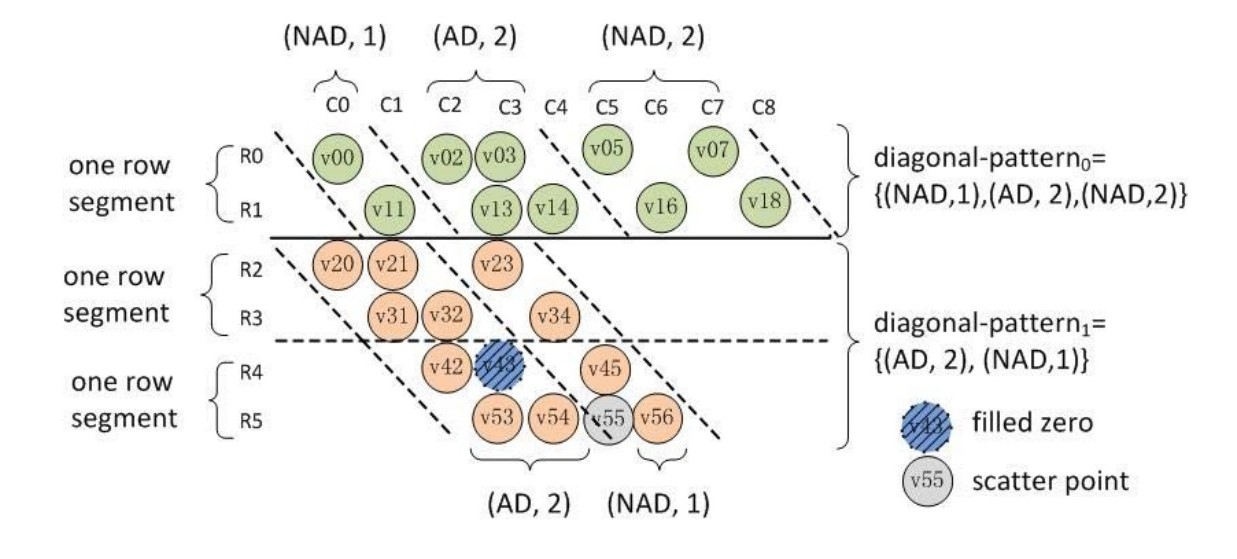
\includegraphics[width=.8\textwidth]{imagenes/chapter3/crsd.jpg}
    \caption{Sección de matriz diagonal, aplicando conceptos del CRSD. Extraído de~\cite{Sun2011}.}
    \label{fig:CRSD}
\end{figure}
Excepto por los elementos más dispersos de la matriz, fuera de diagonales densas, la matriz es almacenada a través de patrones diagonales. Aquellas filas que poseen estos elementos dispersos, o como los denominan los autores scatter point, aquellos que están presentes en una sola diagonal, son agrupadas y almacenadas en forma completa con el formato ELL, debido a que de no utilizar otro formato, sería necesario realizar \textit{zero padding} agregando overhead al procesamiento y trabajo con la matriz. Esta idea puede ser observada mejor en la Figura~\ref{fig:CRSD}.


Otro ejemplo puede ser el formato HYB que combina los formatos ELL y COO, propuesto por Bell y Garland~\cite{Bell2009}. % o modificaciones (mejoras) a formatos existentes dando lugar a formatos nuevos (CoAdELL). 
Este formato busca mitigar ciertas debilidades del esquema ELL, que si bien ofrece ventajas en cuanto a la localidad de datos, es poco eficiente en los casos donde la cantidad de elementos no nulos en cada fila varía considerablemente. En tales circunstancias, 
% con respecto al promedio de este valor por fila, se puede observar que es poco eficiente. Dado el caso, al utilizar este formato se da una caída de desempeño general de los algoritmos, basado en que 
hay un aumento significativo del espacio total requerido (debido al padding necesario para completar los vectores de cada fila con menos de $k$ elementos no nulos, donde $k$ es la cantidad máxima de elementos en una fila de la matriz). Notar además, que los algoritmos operan con estos valores agregados aún siendo nulos.
Para trabajar con estas matrices de forma más eficiente, una opción es utilizar un formato híbrido, que divida la matriz en dos, una componente en formato ELL y la otra por ejemplo en COO. La idea es tener una matriz $A_{ELL}$ de tamaño $n\times k$ donde la cantidad de elementos por fila se aproxime bastante a $k$ y otra matriz $A_{COO}$ para el resto de los elementos. 
% Estas ideas, entre otras, motivaron el formato HYB. %Un ejemplo de matriz dispersa representada en este formato se puede ver en la Figura \ref{fig:hyb-format}.
Elegir la columna $k$ que determine la partición, se puede resolver, como en la implementación de la biblioteca \textit{CUSP}~\cite{cusp-bell}, con una heurística donde dicho valor se elige de forma de que el número de filas con al menos $k$ elementos no nulos, sea menos de un tercio de la cantidad total de filas de la matriz.



Otra investigación donde se combinan dos formatos de almacenamiento de matrices dispersas, enfocadas en mejorar el desempeño de la SpMV en GPUs, se puede encontrar en~\cite{Guo2015}, en la cual Guo et al. presentan ELL and Vectored CSR Hybrid (EVC-HYB). 
El formato presentado se construye primero aplicando reordenamientos simples entre filas basado en los largos de éstas (\nnz por fila), de menor a mayor, y seguido, se realiza una partición en dos grupos, filas largas y cortas. Centrado en esta partición, las entradas de la matriz son almacenadas en los formatos ELL o VCSR\footnote{Vectorized CSR, implementación vectorizada de la SpMV optimizada para GPUs utilizando el formato CSR.} según corresponda. Ambos formatos funcionan bien para ciertos tipos de clases de matrices, por ejemplo, ELL funciona bien con las matrices cuya cantidad de elementos no nulos por fila  es baja y similares entre sí, debido a la localidad de los accesos, en cambio, es muy ineficiente cuando esta cantidad varía considerablemente entre las filas. Mientras que VCSR funciona mejor con matrices cuyas filas son de cierto largo suficiente y en lo posible múltiplos de 32 (warp en GPU), pero la propiedad de los accesos coalesced no puede ser explotada de forma óptima si las filas son de largos menores, particularmente menores a 16. Entonces, buscando aprovechar los beneficios que estos formatos presentan y evitar las debilidades, los autores plantean la estrategia híbrida EVC-HYB que combina ambos. Para la evaluación, en el estudio se comparan contra las mejores elecciones de CUSP para la SpMV, que en general son, CSR y HYB. Evaluaron, para 22 matrices distintas tomadas de la SSMC, la cantidad de operaciones punto flotante por segundo (FLOPS) en 500 iteraciones utilizando los diferentes formatos, obteniendo sin aplicar reordenamientos, mejoras en velocidad de hasta $1,64$, también con resultados que degradaron la cantidad de operaciones, que en el peor de los casos se registraron reducciones en un factor de $0,90$. 

% EL PORQUE DEL HYB (hybrid format propuesto por  Bell and Garland)
% Este formato es poco eficiente cuando la cantidad de elementos no nulos en cada fila varia considerablemente respecto al promedio de elementos no nulos por fila. Dado el caso, hay una pérdida en términos del espacio necesario para almacenar la matriz, asi como 

% Como producto de modificaciones de de formatos existentes, que dieron lugar a estructuras nuevas, a continuación, se estudia el caso del formato 


% CoAdELL, 

% Basado en ELL, formato discutido en~\ref{ell}, se desarrolla CoAdELL, un formato disperso con el que se obtuvo resultados interesantes en la implementación SpMV en GPU. 

% La idea ``innovadora'' , con respecto a su antecesor AdELL, es usar una codificación basada en la distancia entre elementos no nulos. Las distancias entre dos elementos no nulos consecutivos, comunmente, puede ser representada utilizando enteros pequeños, bastando con representaciones de 8-bits o 16 bits para las matrices mas grandes y dispersas.

% AdELL propone, basados en warp gained ELL? (sliced ELL), balancear las cargas entre los warps. Dividiendo la estructura en varias estructuras ELL independientes.....



\section{Múltiples precisiones}\label{multiple-precision}


Operaciones como la SpMV, limitadas por el acceso a memoria~\cite{Goumas2008}, pueden obtener un beneficio inmediato si se logra reducir el uso de memoria en el almacenamiento. El simple hecho de sólo indexar los datos asociados a los elementos no nulos supone una oportunidad para la compresión de estos datos. La mayoría de los formatos dispersos, tienen cierto grado de compresión en los índices. Por ejemplo:  los formatos basados en ELL (ver Sección \ref{ell-format}) no almacenan explícitamente un índice para las filas, sino que este se infiere por la posición en la memoria. Otros formatos en bloque guardan un índice asociado a cada sub-bloque denso (en lugar de almacenar un índice por cada valor no  nulo, reduciendo los datos de indexación) y luego con un desplazamiento acceden a los valores dentro de éste.

El uso de múltiples precisiones es una idea muy empleada en la historia del ALN. En general, centrado en la precisión de los coeficientes de las matrices, tanto por motivos de almacenamiento (por ejemplo trabajar en simple precisión reduce a la mitad el almacenamiento) como de cómputo (en una CPU la relación de desempeño entre simple precisión y doble precisión es 2 a 1 pero en otras plataformas de hardware, como por ejemplo algunas GPUs, las diferencias suelen ser mucho mayores).
En el caso del ALN disperso, es aún mayor la motivación para disminuir la precisión, dado que la principal restricción para el desempeño son los accesos a memoria, por lo que trabajar con precisiones menos demandantes disminuye la cantidad de datos que se mueven por la jerarquía de memorias.

En los últimos años, en el ALN dispersa, han aparecido varios esfuerzos por trabajar con precisiones reducidas o modificaciones de los formatos utilizados. Algunos ejemplos de estos esfuerzos son \cite{Anzt2018, Goebel2020}, donde se evalúa cómo el uso de precisiones reducidas (como half y single) para almacenar algunos coeficientes de los precondicionardores obtenidos con el método de Jacobi, mejora el desempeño al utilizarlos en métodos iterativos para resolver sistemas de ecuaciones lineales.
Específicamente, estos formatos buscan reducir el overhead producido por la transferencia de datos, almacenando adaptativamente los bloques diagonales del precondicionador de Jacobi en distintas precisiones.
En \cite{Grtzmacher2019, Grtzmacher2020} se aplican ideas similares, pero desacoplando el formato de punto flotante utilizado para operaciones aritméticas del formato utilizado para almacenar los datos en la memoria. %, basados en la segmentación o división de la \texttt{mantissa} de los formatos del estándar IEEE,  un formato adaptable de modo que se pueda acceder a los valores con una latencia menor, si se acepta trabajar con una precisión reducida a la hora de obtener resultados, útil para problemas que permiten cierto margen de error o que trabajan con valores acotados.

Un enfoque complementario, es reducir la precisión de los índices asociados a los coeficientes. En este sentido, en el trabajo de Shiming Xu et al. \cite{Xu2010} se propone una optimización de la SpMV, tomando como base el formato ELL, cuyo objetivo es disminuir la cantidad de bits necesarios para representar los índices. En este sentido, se estudia la posibilidad de utilizar como índice de la columna la distancia a la diagonal en lugar del valor real de la coordenada atacando, en este caso, un conjunto acotado de matrices cuadradas de tamaño $n\times n$, donde se busca reducir la distancia de los elementos no-nulos a la diagonal a través de reordenamientos o permutaciones como el método RCM (Reverse Cuthill-McKee). Este trabajo será discutido y analizado con mayor profundidad en la Sección~\ref{sec:reord}.%Habiendo reducido el ancho de banda, proponen la utilización de precisiones reducidas para almacenar los índices.


% \resumen{CoAdELL, utiliza codificacion diferencial, entre dos elementos no nulos de la misma fila}


Otra idea, es la planteada en el formato CoAdELL \cite{Maggioni2014}, donde se continúa la investigación realizada por los mismos autores \cite{AdELL-Maggioni2013}, centrada en la división por warps de los cómputos con matrices almacenadas en formatos basados en ELL. Esta mejora consiste en una técnica de compresión para reducir el almacenamiento asociado a los índices de columna. La idea es utilizar una codificación basada en la diferencia entre los índices de dos elementos no nulos consecutivos en una misma fila, técnica que la mayoría de autores denomina \textit{delta encoding} o \textit{delta compression}, también utilizada con frecuencia en otros campos de estudio~\cite{Ma2010}. Como estas distancias o deltas tendrán valores menores que los índices, se podrán representar con menor cantidad de bits. Por ejemplo, la secuencia 1,~2,~3,~4,~10, de índices de columna, pasa a valer 1,~1,~1,~1,~6. Se intenta entonces, estudiar la posibilidad de una compresión basada en la reducción de precisión de los nuevos coeficientes obtenidos aplicando esta técnica de codificación. %Si bien en el proyecto no se tomó en consideración por cuestiones de practicidad, notar, que esta técnica  puede ser levemente mejorada si se asume un 1 implícito en cada uno de los términos de la secuencia (menos para el primer elemento), dando por resultado la secuencia 1,~0,~0,~0,~5, tal y como se aplica en~\cite{Stevenson2012}.

% Para poder implementar eficientemente estas ideas en hardware masivamente paralelo tiene que ser posible deshacer las convergencias en paralelo. En otras palabras, necesitan la ejecución independiente de los hilos para proporcionar una ejecución adecuada en la GPU. Suponiendo que cada hilo se encarga de procesar, en la SpMV, una entrada del vector $y$, es decir tiene la tarea de computar las sumas y multiplicaciones de una fila de elementos no nulos de la matriz $A$ por las entradas del vector columna $x$.
% Como este hilo sólo procesa sus elementos no nulos, es capaz de calcular el índice de cada entrada a partir de la entrada no nula anterior (implicando, posiblemente, que al menos el primer índice de columna sea almacenado  con una cantidad mayor de bits, por ejemplo 32). %Explican también, que dicha técnica de compresión se acopla  muy bien con estructuras que aplican division por warps, basadas en ELL. Dado un warp en memoria, casi que se puede asumir que cada hilo dentro del warp procesa secuencialmente sus elementos no nulos. 
% Basados en AdELL \cite{AdELL-Maggioni2013}, cada warp está asociado a una estructura ELL ``independiente''. Permitiendo también aplicar de forma selectiva la técnica de compresión por índice de columna a cada warp, dependiendo si todos los delta (diferencias) pueden representarse con 8 o 16 bits. 
% Cabe resaltar que, posiblemente se necesite realizar algún tipo de padding entre el final de un warp ``comprimido'' y el siguiente para garantizar la alineación de 128 bytes.





En otro trabajo, Kourtis et al.~\cite{Kourtis2008} emplean de manera similar la compresión de datos de índice, esta vez buscando reducir la sobrecarga producida
por los mecanismos de descompresión debido a las predicciones erróneas de los flujos de cómputo de la operación. En particular, proponen dos métodos distintos apuntando a comprimir tanto índices como coeficientes no nulos utilizando el formato CSR como base para la investigación, los autores plantean mecanismos para la compresión y descompresión con el objetivo de optimizar la SpMV, atacando primero los índices de columna, estrategia que denominaron CSR Delta Unit (CSR-DU) y luego los coeficientes no nulos con otro formato que llamaron CSR Value Indexed (CSR-VI).  Intentando explotar la distribución por columnas de los elementos no nulos, como se ha estudiado anteriormente utilizan la codificación delta, calculada como la diferencia de índice con respecto al elemento anterior, agregando a esta estrategia la idea de división o agrupamiento por unidades con largos variables, dónde cada una se representa con la cantidad de bits necesaria para el máximo valor de la unidad. Esta compresión trae consigo un cierto overhead en la etapa interna de la SpMV producido por la decodificación dependiendo de la cantidad de bits utilizada. Si los coeficientes fueran comprimidos todos por separado produciría, casi con total seguridad, ramificaciones en la multiplicación, degradando el rendimiento de toda la operación. Entonces, cabe destacar que la decisión de cómo es conformada cada unidad, es decir su tamaño, es de gran impacto en la estrategia. Por ejemplo, si las unidades son muy pequeñas la sobrecarga generada por las divergencias en la descompresión superará a las ganancias que se puedan obtener al comprimir. En cambio, si el tamaño indicado es muy grande, es probable que se encuentren menos oportunidades de compresión debido a que un delta grande impactaría en la cantidad de bits del resto de los índices de la unidad que podrían admitir precisiones menores.


Generalmente, la carga de trabajo de los distintos métodos se concentra en el procesamiento de los valores en punto flotante, ya que normalmente estos se almacenan en doble precisión utilizando 64 bits. Sin embargo, pese a que la ganancia al aplicar compresión es potencialmente mayor, 
% Generalmente, los elementos no nulos de la matriz constituyen la mayor parte del conjunto de trabajo de cuando se utiliza algún formato de compresión, en este caso CSR, principalmente porque requieren 64 bits para ser representados. Por tanto, abordan la compresión desde la premisa de que hay mucho más que ganar con la compresión de los valores que con los índices en términos de reducción del conjunto de trabajo. Sin embargo, 
la compresión de valores en punto flotante no es tan sencilla como la de los números enteros (que permiten en algunos casos reducciones en la cantidad de bits si se conoce los rangos en los que estos trabajan), porque las operaciones aritméticas de punto flotante producen resultados redondeados, y reducir entonces la cantidad de bits implica posiblemente una pérdida de precisión. Pese a esto, los autores indican que existe un número significativo de matrices del conjunto experimental elegido en las que sólo una pequeña parte de sus valores son únicos. Esta redundancia puede ser explotada entonces, almacenando de forma única los valores comunes o repetidos y sus correspondientes referencias o punteros a su ubicación en la matriz, lo que conducirá a la reducción del conjunto de trabajo si la cantidad de valores redundantes es alta en relación al total.  En consecuencia, una reducción considerable en este aspecto, derivará en una mejora del rendimiento en caso de poder compensar el costo derivado de la indirección en el acceso a los valores redundantes.

Las ganancias en desempeño a la hora de utilizar CSR-DU, según los autores,  dependen del porcentaje del tamaño de información de índices sobre el tamaño total de la matriz. En el caso de matrices indexadas con 32-bits que contienen los valores numéricos en 64-bits, el porcentaje es cercano a $1/3$, por lo que la ganancia está limitada por este factor.

% Como se menciona anteriormente, los valores numéricos o coeficientes de la matriz son más difíciles de comprimir debido a principalmente dos razones, la pobre regularidad que éstos presentan y a los límites impuestos por la representación en punto flotante si no se acepta una pérdida de precisión.

Como conclusión general, % en la gran mayoría de las investigaciones se estudia el impacto de la compresión sobre la SpMV. Entonces, 
una técnica de compresión puede ser beneficiosa para la SpMV siempre y cuando el método de descompresión no atosigue al procesador con ramificaciones adicionales irregulares y difíciles de predecir. Como se muestra en~\cite{Goumas2008}, el kernel SpMV es muy sensible a operaciones extra, así como predicciones erróneas en branches pueden fácilmente dañar el desempeño.


Tang et al. \cite{Tang2013} proponen utilizar una familia de esquemas de compresión eficientes, que denominan  \textit{bit-representation optimized} (BRO), para reducir la cantidad de bits requerida para representar los índices. 
% que generalmente contienen una gran cantidad de información redundante, utilizando un formato de representación de bits eficiente. 
En particular, para el diseño de los esquemas de almacenamiento BRO, los autores tomaron en consideración aspectos importantes relacionados con las arquitecturas para las que fueron diseñadas las estrategias. Sin entrar en detalles de implementación, los autores se plantean estudiar el impacto de las etapas necesarias para aplicar estas técnicas. Por ejemplo, para poder realizar la descompresión en GPU, ésta debe ser relativamente liviana en comparación con las operaciones de suma  y multiplicación de la SpMV, de forma que la mayoría de los ciclos de la GPU se asignen a un trabajo útil y no se utilicen únicamente para descomprimir los datos del índice. Además, debido a que las GPU no contienen hardware complejo para la predicción de branches, la descompresión debe evitar los costosas penalizaciones por divergencia dentro de cada warp. 
En este sentido se presentan dos técnicas de compresión de índices, BRO-ELL y BRO-COO, basadas en los formatos ya estudiados ELL y COO, comprimiendo los índices de columna utilizando una codificación delta. La diferencia con otros autores que han trabajado con técnicas similares es que proponen una implementación escalable en GPUs. Por ejemplo, para el caso de BRO-ELL, una vez transformados los vectores de índices de columna en vectores con los delta, sugieren una división de cada uno de éstos en segmentos (llamados slices) de altura $h$. Posteriormente, cada slice es comprimido por un hilo independiente %. Los segmentos, son entonces, asignados a un hilo. Estructuras adicionales son necesarias dado que la cantidad de columnas en cada slice puede variar, por lo que hay que almacenar el largo de cada uno. Posteriormente, los datos de cada segmento se comprimen 
de acuerdo al número de bits necesarios para cada índice delta. Para hacer coincidir el modelo de ejecución SIMT de la GPU y garantizar que el acceso a los datos sea coalesced, se asigna un número fijo de bits para cada columna en un slice con el que se almacenan todos los valores delta de esa columna. Esto requiere encontrar el número máximo de bits necesarios para representar los valores en cada columna, así como estructuras adicionales para almacenar estos valores y la cantidad de columnas en cada slice.

Además de BRO-COO y BRO-ELL, presentan también BRO-HYB, útil en los casos cuando la cantidad de elementos no nulos por filas varía sustancialmente. Este formato es análogo a HYB,  almacenando la componente regular en BRO-ELL y la irregular BRO-COO.


Willcock y Lumsdaine \cite{Willcock2006} desarrollaron dos métodos de compresión sin pérdidas para el formato CSR con el objetivo de reducir el ancho de banda de memoria requerido en la operatoria con matrices dispersas de grandes dimensiones. 
Ambos esquemas de compresión constan de dos etapas: comprimir los índices de una matriz utilizando una cantidad menor de bits antes de almacenar la matriz en la memoria, y descomprimir estos índices sobre la marcha como parte de la SpMV.

En el primer método, \textit{Delta-Coded Sparse Row} (DCSR) se plantea un esquema de compresión basado en la codificación delta de los índices, codificando los índices como las diferencias entre las posiciones de columna de elementos distintos de cero en una fila, utilizando la cantidad mínima de bytes posible. 
Para esto se emplea un conjunto de seis códigos de comando para codificar los datos del índice. 

 El segundo método, \textit{Row Pattern Compressed Sparse Row} (RPCSR), es un enfoque adaptativo que requiere más tiempo de compresión pero cuyo kernel de SpMV presenta un mejor rendimiento. Se basa en fusionar grupos de listas de intervalos de valores delta de los datos de índice. Se lograron aceleraciones de hasta un 30\% respecto a CSR, utilizando el método adaptativo. 
Ninguno de los dos esquemas de compresión presentados cambia los valores numéricos almacenados en la matriz, almacenándolos exactamente en el mismo orden y con la misma precisión que en formato CSR. La investigación está enmarcada en el caso de que la misma matriz se multiplicará repetidamente por muchos vectores, como es el caso de los solvers iterativos de sistemas de ecuaciones o valores propios,
buscando que el tiempo ahorrado por multiplicaciones más rápidas puede compensar el tiempo de compresión.




\section{Reordenamiento}\label{sec:reord}


% Como se dijo anteriormente, los inicios de estas técnicas están relacionados, principalmente, con el afán de almacenar las matrices dispersas como de banda. %Existen tambien multiples investigaciones sobre implmentaciones que aplican reordenamientos para mejorar SpMV

% El principal objetivo de aplicar reordenamientos

% \resumen{el de los chinos}

En la Sección \ref{multiple-precision} se describieron varias estrategias que proponen reducir la precisión con las que trabajan las matrices dispersas con el fin de mejorar la velocidad de los accesos a memoria. Muchas de estas se basan en técnicas como \textit{delta encoding}, que se ve beneficiada cuando los coeficientes no-nulos de la matriz se encuentran en posiciones cercanas entre sí, como sucede en matrices con ancho de banda pequeño. A continuación, se discutirán en más detalle aquellos que proponen aplicar reordenamientos para reducir ancho de banda, mejorar ciertos formatos de almacenamiento, u optimizar de cierta forma la compresión de matrices.


En~\cite{Xu2010}, enfocados en la SpMV, los autores utilizan RCM como método de optimización para la reducción del ancho de banda, %Que como se explicó en la Sección \ref{RCM}, este método intenta, como otras estrategias de reordenamiento, encontrar una permutación expresada como  una matriz $P$ de tal manera que $P A P^t$ tiene los elementos no nulos comprendidos en cierto intervalo (ancho bw) al rededor de la diagonal principal. 
mostrando como la permutación obtenida por el método RCM puede mejorar la localidad de los accesos al vector $x$, además de permitir cierta compresión de la información de columna. 
Dado que $x$ está, en general, expresado como un vector denso y de sólo lectura (read-only), se utiliza el \textit{Texture Cache} (TC) de la GPU para almacenarlo en una memoria de rápido acceso, técnica también utilizada en~\cite{Bell2009,GarlandAndBell2009,Choi2010}.
En el caso del formato ELLPACK, dado que el desplazamiento de los accesos al vector $x$  a la hora de computar la SpMV están indicados por los índices de columna de cada elemento no nulo,  cuando se usa el TC para almacenar $x$, es importante que el patrón de acceso en $x$ tenga las siguientes características de localidad: (1) las direcciones accedidas por hilos (o warps) que se ejecutan cercanos en el tiempo sean cercanos en memoria, y (2) direcciones accedidas por un hilo en iteraciones consecutivas sean cercanas. El primer punto, requiere que los hilos dentro del mismo ThreadBlock (TB) posean direcciones similares, es decir, las filas adyacentes deben tener patrones de dispersión similares. El segundo requiere que los elementos no nulos en una fila deben estar lo más juntos posibles, es decir, agrupados en ciertas posiciones. Esto implica que permutaciones matriciales que mejoran las estructuras locales y generan bloques más densos pueden resultar en un mejor aprovechamiento del principio de localidad a la hora de acceder a $x$. Los autores utilizan el método RCM para mejorar la localidad. Para matrices de ancho de banda reducido luego de aplicar RCM, existe un buen límite superior para las regiones a las que accede cada TB: T + BW, donde T es el número de hilos por TB y BW es el ancho de banda de la matriz. En caso de que el ancho de banda no se reduzca de manera efectiva, RCM también tiende a generar filas con patrones de dispersión similares agregando elementos no nulos al perfil exterior de la matriz, debido a que la heurística inmediatamente luego de procesar un vértice procesa los vecinos, provocando que estas aristas aumenten el ancho de banda, pero sobre la misma columna. Esto corresponde a una mejora de la localidad espacial para threads adyacentes.


La reducción del ancho de banda de la matriz permite también %en algunos casos,
la compresión de los índices para acceder a la información. Es decir, al pasar a una matriz de banda, hay una gran correlación entre los índices de fila y columna, $r$  y $c$ para cada elemento no nulo de la matriz. Además, se puede verificar que hay una diferencia de como máximo $BW/2$ entre ambos valores. Visto de otra forma los índices de fila y columna cumplen que: $r - BW/2 \leq c \leq r + BW/2$. Los autores proponen guardar la distancia del elemento hacia la diagonal en lugar de los índices de columna para matrices con anchos de banda reducidos. % En el esquema en lugar del valor de columna $c$, se plantea almacenar $(c - r)$, i.e., el offset o 
 Dada la reducción del ancho de banda, $BW$ tiende a ser pequeño, permitiendo así expresar $(c -r)$ con menor cantidad de bits. Notar que, como contrapartida, es necesario utilizar un formato de numeración con signo, dado que las entradas que están por debajo de la diagonal, tendrán un offset negativo, a diferencia de cuando se almacenaba $c$ que permitía el uso de formatos sin signo. Los autores proponen utilizar una representación de 16-bits para almacenar la diferencia $(c -r)$, estudiando cuáles matrices del conjunto de prueba elegido aplican para la compresión de índice.
 
Para la evaluación, los autores evalúan y comparan la velocidad de los accesos a las matrices, almacenadas aplicando la estrategia propuesta para SP y DP, y a los vectores $x$ en la operación SpMV. En promedio, para matrices con ancho de banda reducido, se logra una reducción del 26\% y 33\% en el tiempo requerido para acceder al vector $x$. El ancho de banda reducido también permite la compresión del índice de columna utilizando precisiones reducidas, lo que resulta en una reducción del 25\% (para SP) y del 16\% (para DP) en el tiempo requerido para acceder a los datos de la matriz. En promedio, se alcanzan para SP y DP, 16\% y 12,6\% respectivamente, en todo el conjunto de prueba conformado por 11 matrices bien conocidas y utilizada en otras investigaciones~\cite{Bell2009}.


En la literatura se han utilizado métodos de reordenamiento de matrices como el algoritmo RCM para reducir el ancho de banda de la matriz y disminuir el número de elementos no-nulos que se generan al aplicar la factorización LU o Cholesky. En \cite{Pinar1999} Pinar y Heath, proponen estructuras alternativas de almacenamiento para matrices dispersas, junto con algoritmos de reordenamiento para incrementar la efectividad de dichas estructuras, con el principal objetivo de reducir la cantidad de accesos indireccionados. Dicho de otra forma, un reordenamiento es aplicado para permutar los elementos no nulos de la matriz, llevándolos a ubicaciones contiguas, tanto como sea posible, para agrandar los bloques densos. 
En este contexto, presentan dos estrategias de almacenamiento basadas en bloques, cuya efectividad depende directamente de la disponibilidad de bloques densos. La primera presenta la idea de trabajar con la matriz dispersa expresada como la suma de varias matrices. En particular, descomponen la matriz original en dos matrices, donde una contiene bloques densos de tamaño fijo $r \times c$ (en el caso del trabajo en cuestión $1\times 2$), y la otra con los restantes elementos. El uso de estos bloques densos puede reducir el número total de operaciones de carga, así como el total de memoria requerida. Dado que el tamaño de los bloques es fijo, sólo un índice es necesario para direccionar un bloque. La segunda estrategia de almacenamiento abordada también utiliza bloques, pero a diferencia de la anterior, éstos son de largo variable, permitiendo así empaquetar más elementos no nulos en un solo bloque. De nuevo, la ventaja que ofrecen estas estructuras es que sólo es necesario el índice del primer elemento no nulo del bloque para acceder a los elementos contiguos. %Es decir, que es necesario un acceso de memoria para acceder a todos los elementos de un bloque. 
Esta estrategia reduce la cantidad de operaciones de carga de índices, pero requiere un ciclo más en la SpMV generando cierto overhead. Debido a esto, la elección del tamaño de los bloques afecta directamente la efectividad del método, si el tamaño de los bloques es muy pequeño la sobrecarga generada por el ciclo extra dominará sobre la ganancia de reducir la cantidad de operaciones de carga.

Dado que el desempeño de estos métodos se encuentra ligado a la existencia de bloques densos, se propone aplicar reordenamientos con el objetivo de mejorar dicho aspecto. 
Los autores demuestran que el problema de reordenar las columnas es $\mathcal{NP}$-completo y, por lo tanto, se deben utilizar heurísticas para obtener una solución práctica. Proponen entonces, un modelo basado en el Travelling Salesperson Problem (TSP)~\cite{reinelt1994}, usando heurísticas diseñadas para ese problema. Notar que los casos de estudio, TSP y reordenar la matriz, no corresponden directamente al mismo problema, ya que mientras que uno busca encontrar un ciclo o un camino cerrado, el otro busca solamente un camino que pase por todos los nodos. 
Utilizando esta estrategia se intenta encontrar el recorrido que maximice el peso del camino. Para esto definieron el peso de una arista como la cantidad de filas que tienen elementos no nulos en las columnas correspondientes a los vértices unidos por esa arista. Los autores muestran que las  estructuras de datos y técnicas de reordenamiento presentadas producen mejoras de hasta un 33\% y mejoras de un 21\% en promedio.

En otra investigación, Monakov et al.~\cite{Monakov2010} proponen, con el objetivo de mejorar el rendimiento de la SpMV en GPUs, un nuevo formato que denominaron sliced ELLPACK. Este formato tiene por parámetro principal $S$, que es el tamaño o la cantidad de filas de cada \textit{slice}. Cada una de estas porciones o slices es almacenada en formato ELL.  
Si bien la sobrecarga de almacenamiento en el formato sliced ELLPACK se limita a los slices con un desequilibrio en el número de elementos no-nulos por fila, esto aún puede causar una degradación notable del rendimiento. Los autores proponen entonces, una heurística simple de reordenamiento que puede mejorar sustancialmente la performance de la implementación de la SpMV para el formato presentado. Esta se basa en reordenar las filas agrupando aquellas con el mismo número de elementos distintos de cero. %(Parecido a CoAdELL, esto es mas viejo).
Es importante destacar, sin entrar en detalles, que los autores tuvieron en cuenta la complejidad del algoritmo de reordenamiento, proponiendo uno lineal en el número de filas de la matriz. 
De forma breve, la heurística consiste en un mecanismo simple de $B$ cubetas (\textit{buckets}), numeradas de $0$ a $B - 1$, donde la cubeta $z$ contiene las filas con $z$ elementos, y aquellas filas con más de $B$ elementos son asignadas a la última cubeta. Si al agregar una fila a una cubeta ésta alcanza las $S$ filas, se vacía dicha cubeta agregando las filas agrupadas a la matriz reordenada formando un slice con $z$ elementos en cada fila. Esto se repite hasta recorrer todas las filas, y las restantes que aún no hayan sido agregadas a la matriz reordenada se agregan de forma arbitraria.
A partir de la etapa experimental muestran que esta heurística simple puede mejorar en gran medida el rendimiento. 


Con el objetivo de aprovechar los métodos de compresión, los mismos autores de~\cite{Tang2013} extienden sus primeras propuestas con el uso de una estrategia de ordenamiento que denominaron \textit{BRO-aware reordering} (BAR). Esta estrategia consiste en acercar aquellas columnas que poseen patrones similares en cuanto a la cantidad de bits necesarios para su codificación, de modo de reducir el espacio total y, en consecuencia, reducir posiblemente el número de transacciones a la hora de operar con la matriz. La obtención de la permutación $P$, es formulada por los autores como un problema de clusterización. Consiste en encontrar $v$ particiones iguales disjuntas entre sí del conjunto de filas $\mathcal{R}$ expresadas con los delta, minimizando el número de transacciones requeridas por la SpMV. Con este objetivo, plantean una serie de ecuaciones y funciones a minimizar e indican que una posible limitante de este problema es que la forma de clusterización elegida toma en cuenta sólo la localidad espacial, y no la temporal. En general, es sabido que encontrar la solución óptima global para problemas de este estilo es $\mathcal{NP}$-completo~\cite{Jain2010}. Proponen, entonces, una heurística greedy para particionar las filas de la matriz. 
La evaluación experimental muestra que \textit{BRO-aware} obtuvo mejor desempeño y ahorro de memoria, luego de comprimir la matriz en formato BRO-ELL, que AMD\footnote{El Approximate Minimum Degree (AMD)~\cite{George1989} es un algoritmo de reordenamiento para matrices simétricas, utilizado generalmente, para reducir la cantidad de \textit{fill in} producido en la factorización, por ejemplo, de Cholesky.} y RCM en la mayoría de los casos. 
%En cuanto a los resultados del reordenamiento, comparado con RCM y AMD, aplicados sobre BRO-ELL, se obtuvo que \textit{BRO-aware} obtuvo en la mayoría de los casos resultados resultados mejores, tanto en desempeño, con un máximo de 7\% comparado con BRO-ELL original, como en espacio ahorrado. 
En promedio con BAR se obtuvieron ahorros en el espacio de almacenamiento de 4\%, comparados contra un 1\% para RCM y AMD. Cabe destacar que el algoritmo greedy presentado puede que no llegue a soluciones de buena calidad siempre. Por ejemplo, para un caso (la matriz \textit{cant}) RCM y AMD obtuvieron mejores resultados que BAR, debido principalmente a que no se toma en cuenta la localidad temporal, lo que genera muchas veces, múltiples fallas en el uso del caché.


Con el creciente uso del Aprendizaje Automático en múltiples ámbitos, y la capacidad de cómputo que estos necesitan, han surgido varios estudios que buscan la forma de optimizar operaciones como SpMM (Sparse-dense Matrix Multiplication) y SDDMM (Sampled Dense Dense Matrix Multiplication), frecuentes en este tipo de estrategias. Un estudio de este estilo es el presentado por Hong et al.~\cite{Hong2019}, en dicho artículo se diseña una estrategia de ordenamiento basada en \textit{tiling} adaptativo, aplicándola para mejorar el rendimiento de las dos primitivas, SpMM y SDDMM. 
El \textit{tiling} es una técnica muy importante para la optimización de la localidad de datos. Consiste en agrupar elementos de la matriz en bloques o tiles, generalmente 2D, con los cuales se realiza cierta operación, por ejemplo multiplicaciones y convoluciones.  Usada ampliamente en implementaciones de alto rendimiento de multiplicaciones matriz-matriz densas, tanto para CPU y GPU, que aplicando un \textit{tiling} uniforme, todos los \textit{tiles}, sin ser aquellos ubicados en los bordes, necesitan la misma cantidad de transferencia de datos, como operaciones.  Sin embargo, el irregular patrón de acceso a datos dependiente de las matrices dispersas en la multiplicaciones dificulta el uso del \textit{tiling} para mejorar la reutilización de datos. A continuación se presenta un breve resumen de los resultados obtenidos en~\cite{Hong2019} con la estrategia propuesta, Adaptive Spaese Tiling (ASpT).  Los autores proponen, a diferencia de otras investigaciones similares que utilizan formatos particulares y personalizados para optimizar las operaciones, una implementación utilizando un formato estándar, en este caso CSR. Posiblemente una de las razones más importantes por las cuales es bueno utilizar un formato estándar como CSR es la compatibilidad con el código y las bibliotecas existentes. 
La idea es que el número medio de no ceros por segmento de fila/columna ``activo'' (es decir, al menos uno elemento no nulo) dentro de un bloque 2D juega un papel importante en la determinación de si es preferible para dicho bloque la ejecución aplicando \textit{tiling} o no.
\begin{figure}[h]
    \centering
    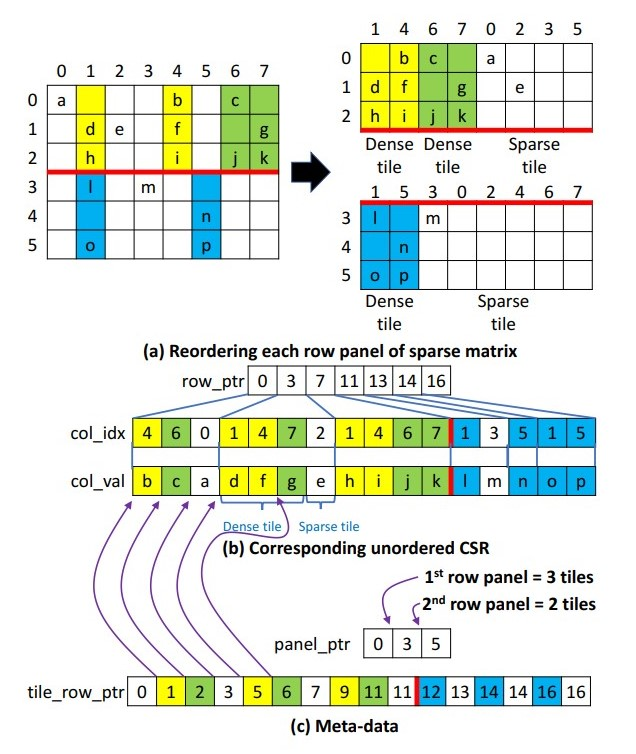
\includegraphics[width=.7\textwidth]{imagenes/chapter3/aspt_csr.jpg}
    \caption{Modificación de CSR con reordenamiento. Extraída de~\cite{Hong2019}.}
    \label{fig:aspt_csr}
\end{figure}
Entonces, la matriz dispersa se divide en paneles de filas, y las columnas activas dentro de cada panel de filas son agrupadas en tiles 2D para la ejecución o se relegan a la ejecución sin \textit{tiling} porque su densidad de columna ``activa'' es inadecuada. La propiedad adaptativa del \textit{tiling} en ASpT viene dada por la combinación el formato CSR con un reordenamiento dentro de las filas, buscando mejorar la localidad de los accesos. Se diferencian de otros autores por utilizar un reordenamiento que no produce tanta sobrecarga como las estrategias clásicas basadas en algoritmos greedy para grafos. Además, la técnica propuesta reordena sólo los elementos no nulos manteniendo una estructura auxiliar y no renumera todo el grafo, es decir, los índices de los elementos para el formato CSR se mantienen. La idea principal es numerar los vértices de modo que a los vértices con muchos vecinos comunes se les asignen índices cercanos entre sí para mejorar la localidad de los accesos. Se puede observar mejor en la Figura~\ref{fig:aspt_csr}.

